\chapter{Exodus 34}

\begin{figure}
  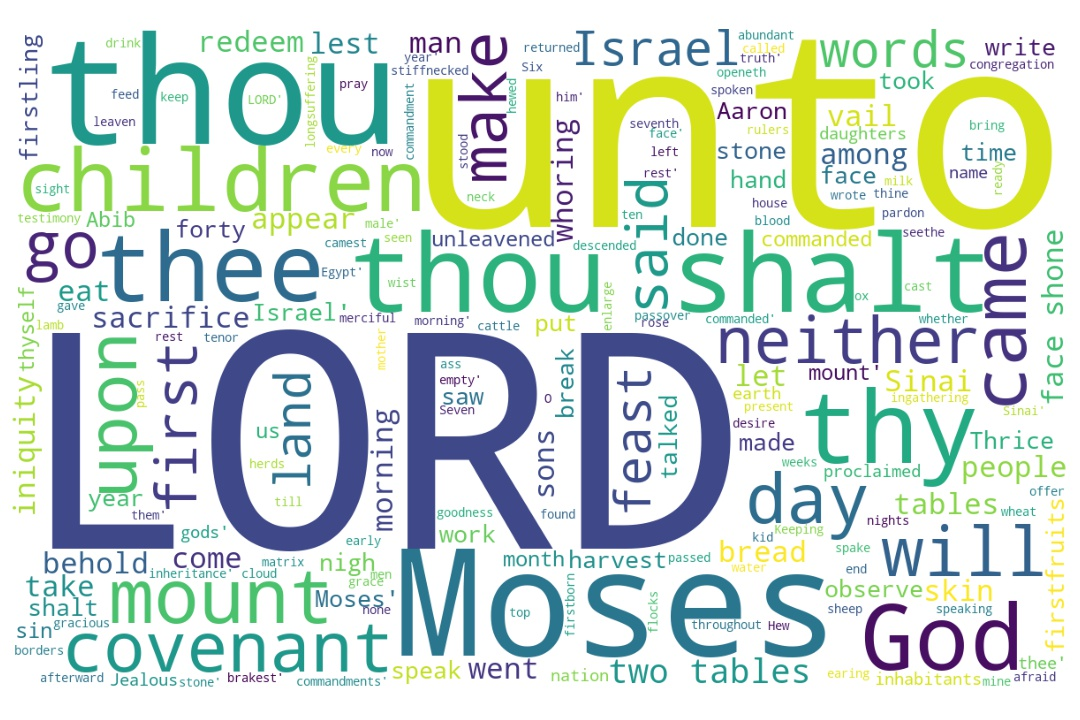
\includegraphics[width=\linewidth]{02OT-Exodus/Exodus34-WordCloud.jpg}
  \caption{Exodus 34 Word Cloud}
  \label{fig:Exodus 34 word Cloud}
\end{figure}



\marginpar{\scriptsize \centering \fcolorbox{bone}{lime}{\textbf{BE READY}}\\ (Exodus 34:1-35) \begin{compactenum}[I.][8]
    \item To \textbf{Receive Instruction} from God \index[scripture]{Exodus!Exo 34:02}(Exodus 34:2)
    \item To be \textbf{Visited} by God\index[scripture]{Exodus!Exo  19:11}(Exo 19:11)
    \item To be \textbf{Rescued} by God \index[scripture]{Esther!Est 08:13}(Est 8:13)
    \item For a \textbf{Revelation} \index[scripture]{Job!Job 18:12}(Job 18:12)
    \item To \textbf{Reject} False gods \index[scripture]{Daniel!Dan 03:15}(Dan 3:15)
    \item To \textbf{Render} Gifts \index[scripture]{2 Corinthians!2Cor 09:03}\index[scripture]{2 Corinthians!2 Corinthians 09:05}(2 Cor 9:3, 5)
   \item To \textbf{Respond} for God \index[scripture]{1 Peter!1Pet 03:15}(1 Pet 3:15)
%    \item A \textbf{Service} \index[scripture]{Exodus!Exodus 27:19}(Exodus 27:19)
%    \item A \textbf{Statute} \index[scripture]{Exodus!Exodus 27:21}(Exodus 27:21)
%    \item The \textbf{Sons} \index[scripture]{Exodus!Exodus 27:21}(Exodus 27:21)
\end{compactenum}}

%%%%%%%%%%%%%%%%%%%%%%%%%%%%%%%%%%%%%%
%%%%%%%%%%%%%%%%%%%%%%%%%%%%%%%%%%%%%
\footnote{\textcolor[cmyk]{0.99998,1,0,0}{\hyperlink{TOC}{Return to end of Table of Contents.}}}\footnote{\href{https://audiobible.com/bible/exodus_34.html}{\textcolor[cmyk]{0.99998,1,0,0}{Exodus 34 Audio}}}\textcolor[cmyk]{0.99998,1,0,0}{And \fcolorbox{bone}{bone}{the LORD} said unto \fcolorbox{bone}{bone}{Moses}, Hew thee two tables of stone like unto the first: and I will write upon \emph{these} tables the words that were in the first tables, which thou brakest.}
[2] \textcolor[cmyk]{0.99998,1,0,0}{And \fcolorbox{bone}{lime}{be ready} in the morning, and come up in the morning unto mount Sinai, and present thyself there to me in the top of the mount.}
[3] \textcolor[cmyk]{0.99998,1,0,0}{And no man shall come up with thee, neither let any man be seen throughout all the mount; neither let the flocks nor herds feed before that mount.}\\
\\
\P \textcolor[cmyk]{0.99998,1,0,0}{And he hewed two tables of stone like unto the first; and \fcolorbox{bone}{bone}{Moses} rose up early in the morning, and went up unto mount Sinai, as \fcolorbox{bone}{bone}{the LORD} had commanded him, and took in his hand the two tables of stone.}
[5] \textcolor[cmyk]{0.99998,1,0,0}{And \fcolorbox{bone}{bone}{the LORD} descended in the cloud, and stood with him there, and proclaimed the name of the LORD.}
[6] \textcolor[cmyk]{0.99998,1,0,0}{And \fcolorbox{bone}{bone}{the LORD} passed by before him, and proclaimed, The LORD, \fcolorbox{bone}{bone}{the LORD} God, merciful and gracious, longsuffering, and abundant in goodness and truth,}
[7] \textcolor[cmyk]{0.99998,1,0,0}{Keeping mercy for thousands, forgiving iniquity and transgression and sin, and that will by no means clear \emph{the} \emph{guilty}; visiting the iniquity of the fathers upon the children, and upon the children's children, unto the third and to the fourth \emph{generation}.}
[8] \textcolor[cmyk]{0.99998,1,0,0}{And \fcolorbox{bone}{bone}{Moses} made haste, and bowed his head toward the earth, and worshipped.}
[9] \textcolor[cmyk]{0.99998,1,0,0}{And he said, If now I have found grace in thy sight, O Lord, let my Lord, I pray thee, go among us; for it \emph{is} a stiffnecked people; and pardon our iniquity and our sin, and take us for thine inheritance.}
[10] \textcolor[cmyk]{0.99998,1,0,0}{And he said, Behold, I make a covenant: before all thy people I will do marvels, such as have not been done in all the earth, nor in any nation: and all the people among which thou \emph{art} shall see the work of the LORD: for it \emph{is} a terrible thing that I will do with thee.}
[11] \textcolor[cmyk]{0.99998,1,0,0}{Observe thou that which I command thee \fcolorbox{bone}{lime}{this day}: behold, I drive out before thee the Amorite, and the Canaanite, and the Hittite, and the Perizzite, and the Hivite, and the Jebusite.}
[12] \textcolor[cmyk]{0.99998,1,0,0}{Take heed to thyself, lest thou make a covenant with the inhabitants of the land whither thou goest, lest it be for a snare in the midst of thee:}
[13] \textcolor[cmyk]{0.99998,1,0,0}{But ye shall destroy their altars, break their images, and cut down their groves:}
[14] \textcolor[cmyk]{0.99998,1,0,0}{For thou shalt worship no other god: for  \fcolorbox{bone}{bone}{the LORD} , whose name \emph{is} Jealous, \emph{is} a jealous God:}
[15] \textcolor[cmyk]{0.99998,1,0,0}{Lest thou make a covenant with the inhabitants of the land, and they go a whoring after their gods, and do sacrifice unto their gods, and \emph{one} call thee, and thou eat of his sacrifice;}
[16] \textcolor[cmyk]{0.99998,1,0,0}{And thou take of their daughters unto thy sons, and their daughters go a whoring after their gods, and make thy sons go a whoring after their gods.}
[17] \textcolor[cmyk]{0.99998,1,0,0}{Thou shalt make thee no molten gods.}\\
\\
\P \textcolor[cmyk]{0.99998,1,0,0}{The feast of unleavened bread shalt thou keep. Seven days thou shalt eat unleavened bread, as I commanded thee, in the time of the month Abib: for in the month Abib thou camest out from Egypt.}
[19] \textcolor[cmyk]{0.99998,1,0,0}{All that openeth the matrix \emph{is} mine; and every firstling among thy cattle, \emph{whether} ox or sheep, \emph{that} \emph{is} \emph{male}.}
[20] \textcolor[cmyk]{0.99998,1,0,0}{But the firstling of an ass thou shalt redeem with a lamb: and if thou redeem \emph{him} not, then shalt thou break his neck. All the firstborn of thy sons thou shalt redeem. And none shall appear before me empty.}\\
\\
\P \textcolor[cmyk]{0.99998,1,0,0}{Six days thou shalt work, but on the seventh day thou shalt rest: in earing time and in harvest thou shalt rest.}\\
\\
\P \textcolor[cmyk]{0.99998,1,0,0}{And thou shalt observe the feast of weeks, of the firstfruits of wheat harvest, and the feast of ingathering at the year's end.}\\
\\
\P \textcolor[cmyk]{0.99998,1,0,0}{Thrice in the year shall all your men children appear before \fcolorbox{bone}{bone}{the LORD} GOD, the God of Israel.}
[24] \textcolor[cmyk]{0.99998,1,0,0}{For I will cast out the nations before thee, and enlarge thy borders: neither shall any man desire thy land, when thou shalt go up to appear before \fcolorbox{bone}{bone}{the LORD} thy God thrice in the year.}
[25] \textcolor[cmyk]{0.99998,1,0,0}{Thou shalt not offer the blood of my sacrifice with leaven; neither shall the sacrifice of the feast of the passover be left unto the morning.}
[26] \textcolor[cmyk]{0.99998,1,0,0}{The first of the firstfruits of thy land thou shalt bring unto the house of \fcolorbox{bone}{bone}{the LORD} thy God. Thou shalt not seethe a kid in his mother's milk.}
[27] \textcolor[cmyk]{0.99998,1,0,0}{And \fcolorbox{bone}{bone}{the LORD} said unto \fcolorbox{bone}{bone}{Moses}, Write thou these words: for after the tenor of these words I have made a covenant with thee and with Israel.}
[28] \textcolor[cmyk]{0.99998,1,0,0}{And he was there with \fcolorbox{bone}{bone}{the LORD} forty days and forty nights; he did neither eat bread, nor drink water. And he wrote upon the tables the words of the covenant, the ten commandments.}\\
\\
\P \textcolor[cmyk]{0.99998,1,0,0}{And it came to pass, when \fcolorbox{bone}{bone}{Moses} came down from mount Sinai with the two tables of testimony in Moses' hand, when he came down from the mount, that \fcolorbox{bone}{bone}{Moses} wist not that the skin of his face shone while he talked with him.}
[30] \textcolor[cmyk]{0.99998,1,0,0}{And when Aaron and all the children of Israel saw \fcolorbox{bone}{bone}{Moses}, behold, the skin of his face shone; and they were afraid to come nigh him.}
[31] \textcolor[cmyk]{0.99998,1,0,0}{And \fcolorbox{bone}{bone}{Moses} called unto them; and Aaron and all the rulers of the congregation returned unto him: and \fcolorbox{bone}{bone}{Moses} talked with them.}
[32] \textcolor[cmyk]{0.99998,1,0,0}{And afterward all the children of Israel came nigh: and he gave them in commandment all that \fcolorbox{bone}{bone}{the LORD} had spoken with him in mount Sinai.}
[33] \textcolor[cmyk]{0.99998,1,0,0}{And \emph{till} \fcolorbox{bone}{bone}{Moses} had done speaking with them, he put a vail on his face.}
[34] \textcolor[cmyk]{0.99998,1,0,0}{But when \fcolorbox{bone}{bone}{Moses} went in before \fcolorbox{bone}{bone}{the LORD} to speak with him, he took the vail off, until he came out. And he came out, and spake unto the children of Israel \emph{that} which he was commanded.}
[35] \textcolor[cmyk]{0.99998,1,0,0}{And the children of Israel saw the face of \fcolorbox{bone}{bone}{Moses}, that the skin of Moses' face shone: and \fcolorbox{bone}{bone}{Moses} put the vail upon his face again, until he went in to speak with him.}